
This chapter covers the theoretical background for the research presented in this thesis. Starting with the description of the Standard Model, this chapter will analyze its limits and suggest one possible theoretical extension, supersymmetry. This additional theory can explain some of the phenomena in nature that the Standard Model cannot describe.

\section{The Standard Model of Particle Physics}

The Standard Model of particle physics is a theory that describes three of the forces existing in nature, the electromagnetic, the weak and the strong force and defines the fundamental constituents of matter \cite{Spiesberger:2000ks}. It was developed in the second half of the century as combined theoretical and experimental effort by the research communities from all around the world. Since the first formulation at the beginning of the 1970s the Standard Model successfully predicted all the particles that were discovered later in the century. The most recent particle discoveries such as the top quark (1995), the tauonic neutrino (2000) and finally the Higgs boson (2012) have given further credence to the Standard Model. 

According to this theoretical model the basic constituents of matter are leptons and quarks, which are divided into three families of identical structure. \autoref{table:fermions} shows all the fermions of the Standard Model and their charges, arranged in the three families. Details on the main aspects of this theory are gonna be given in the following sections.

\begin{figure}[tbh!]
	\begin{center}
		
		\begin{tabular}{ | c | c | c | c | c |}
			\hline
			& 1st Generation & 2 Generation & 3rd Generation & charge \\ \hline \hline
			& & & & \\
			leptons & $\left( \begin{array}{c} \nu_{e} \\ e \end{array} \right)_{\text{L}}$ & $\left( \begin{array}{c} \nu_{\mu} \\ \mu \end{array} \right)_{\text{L}}$ & $\left( \begin{array}{c} \nu_{\tau} \\ \tau \end{array} \right)_{\text{L}}$ & \begin{tabular}{@{}c@{}}weak \\ weak, electromagnetic\end{tabular} \\
			& & & & \\
			& $e_{\text{R}}$& $\mu_{\text{R}}$& $\tau_{\text{R}}$& electromagnetic\\ 
			& & & & \\
			\hline
			& & & & \\
			quarks & $\left( \begin{array}{c} u \\ d \end{array} \right)_{\text{L}}$ & $\left( \begin{array}{c} c \\ s \end{array} \right)_{\text{L}}$ & $\left( \begin{array}{c} t \\ b \end{array} \right)_{\text{L}}$ & weak, electromagnetic, strong \\
			& & & & \\
			& $u_{\text{R}}, d_{\text{R}}$& $c_{\text{R}}, s_{\text{R}}$& $t_{\text{R}}, b_{\text{R}}$& electromagnetic, strong\\
			& & & & \\ 
			\hline
			\hline
		\end{tabular}
		\caption{Fermions of the Standard Model and their charges, arranged in the three generations. Only the left-handed fermions interact weakly and are arranged in doublets. The right-handed fermions are singlets. The right-handed neutrinos are not present in this table, as they do not interact with one of the forces of the Standard Model.}
		\label{table:fermions}
	\end{center}
\end{figure}

\subsection{The Higgs Mechanism}
\label{higgs_mechanism}

The discovery of the Higgs boson led to the confirmation of a mechanism that was developed in 1964 to solve the problem of a symmetric Lagrangian with massless particles which did not agreed with experimental evidence. This mechanism works by introducing a new gauge boson and spontaneously breaking symmetry.

The starting point is moving from a global gauge transformation to a point-dependent gauge transformation applied to the minimal Lagrangian $\mathcal{L}$. This requires in addition to the starting complex scalar field $\phi$ also a vectorial field $A_{\mu}$ analog to the electromagnetic field. The resulting Lagrangian is:

\begin{equation}
\mathcal{L} = (D_{\mu}\phi)^{\dagger} D^{\mu}\phi - V (\phi) - \dfrac{1}{4}F_{\mu\nu}F^{\mu\nu}\
\label{eq::lagrangian_min}
\end{equation}

where $V(\phi)$ is the $\phi$ field potential:

\begin{equation}
V(\phi)=\mu^{2}\phi^{\dagger}\phi+\lambda(\phi^{\dagger}\phi)^{2} -\epsilon\phi^{\dagger} -\epsilon^{*}\phi
\end{equation}

$D^{\mu}$ is the covariant derivative:

\begin{equation}
D^{\mu} = \partial^{\mu} - ieA^{\mu},
\end{equation}

and $F^{\mu\nu}$ is the tensor of the vector field $A_{\mu}$:

\begin{equation}
F^{\mu\nu} =\partial^{\nu}A^{\mu} - \partial^{\mu}A^{\nu}.
\end{equation}

where $\epsilon \rightarrow 0$, $\mathcal{L}$ is invariant under gauge transformations:

\begin{equation}
\phi(x) \rightarrow e^{i\alpha(x)}\phi(x); \phi(x)^{\dagger} \rightarrow e ^{-i\alpha(x)}\phi(x)^{\dagger}
\end{equation}

\begin{equation}
A^{\mu} \rightarrow A^{\mu} + \dfrac{1}{e}\partial^{\mu}\alpha(x)
\label{eq::a_tranform}
\end{equation}

where $\alpha(x)$ is an arbitrary function of x and $e$ is a new coupling constant, identical to the electric charge in case $A_{\mu}$ is identified as the electromagnetic field. In order to obtain a stable theory $\lambda > 0$, however $\mu^{2}$ can have two cases depending on the sign choice:
 
1. $\mu^{2} > 0$. The energy minimum is at $\phi = 0$ and $A_{\mu} = 0$. The resulting theory consists of:

\begin{enumerate}
	\item a charged particle and its anti-partner, both with mass $\mu^{2} \neq 0$;
	\item a massless particle with spin 0, similar to the photon.
\end{enumerate}

For small values of $\lambda$ and $e$ the Lagrangian describes the interactions between scalar particles with the electromagnetic field (trough the coupling constant $e$) and their self-interactions (through the couping constant $\lambda$).

2. $\mu^{2} < 0$. The energy minimum is at $A_{\mu} = 0$, so in  case $\epsilon \rightarrow 0$:

\begin{equation}
V(\bar{\phi}) = \text{min }; \quad \bar{\phi}=\eta= 2\lambda +O(\epsilon)
\end{equation}
 
 in order to study the  variations around the minimum $\phi$ is defined as:

\begin{equation}
 \phi=\eta + \dfrac{\sigma_{1}(x) + i\sigma_{2}(x)}{\sqrt{2}} 
\end{equation}

and is used into the minimal Lagrangian \ref{eq::lagrangian_min}.

The particle masses spectrum is obtained from the fields $\sigma_{i}$ and $A_{\mu}$ quadratic terms. In addition, for $\alpha \rightarrow 0$, $\phi$ transforms as:

\begin{equation}
\phi \rightarrow \phi + i\alpha\phi = \eta + \dfrac{\sigma_{1}(x) + i\sigma_{2}(x)}{\sqrt{2}} + i\eta\alpha(x)
\end{equation}

or rather:

\begin{equation}
\sigma_{1}(x) \rightarrow \sigma^{\prime}_{1}(x) = σ_{1}(x); \quad \sigma_{2}(x) \rightarrow \sigma^{\prime}_{2}(x) = \sigma_{2}(x) + \sqrt{2}\eta\alpha(x)
\end{equation}

$A_{\mu}$ transforms following \autoref{eq::a_tranform}. The $\sigma_{2}$ field non-homogeneously transforms by the addition of an $\alpha$ term, arbitrary function of $x$. In case of the given $\sigma_{i}(x)$ and $A_{\mu}$ where:

\begin{equation}
\alpha(x) = -\dfrac{σ\sigma_{2}(x)}{\sqrt{2}\eta}
\end{equation}

resulting in:

\begin{equation}
\sigma^{\prime}_{2}(x) = 0
\label{eq::unitary_gauge}
\end{equation}

the $\sigma_{2}$ filed can be crossed out in case of a gauge symmetry. The gauge identified by \autoref{eq::unitary_gauge} is commonly known as unitary gauge.

\subsection{The bosonic masses}

The starting point is the electroweak Lagrangian $\mathcal{L}_{\text{eW}}$ based on the $\text{SU}(2)_{\text{L}} \oplus \text{U}(1)_{\text{Y}}$ symmetry:

\begin{equation}
\mathcal{L}_{\text{eW}} = \bar{l}i\gamma^{\mu} D_{\mu}l + \bar{e}_{\text{R}}i\gamma^{\mu}D_{\mu}e_{\text{R}} - \dfrac{1}{4}[W_{\mu\nu}W^{\mu\nu} +B_{\mu\nu}B^{\mu\nu}]
\label{eq::lagrangian_ew}
\end{equation}

with the leptonic fields defined as:

\begin{equation}
\binom{(\nu_{e})_{\text{L}}}{e_{\text{L}}}_{\text{Y}=−2} ; \quad (e_{\text{R}})_{\text{Y}=−2}
\label{eq::fields_scheme}
\end{equation}

and the covariant derivatives and tensors defined as:

\begin{equation}
D_{\mu}l = [\partial_{\mu} + igW_{\mu} \dfrac{\tau}{2}  + ig^{\prime}(-\dfrac{1}{2})B_{\mu}]l 
\end{equation}

\begin{equation}
D_{\mu}e_{\text{R}} = [\partial_{\mu} + ig^{\prime}(-1)B_{\mu}]e_{\text{R}}
\end{equation}

\begin{equation}
W_{\mu\nu} =\partial_{\nu}W_{\mu} - \partial_{\mu}W_{\nu} 
\end{equation}

\begin{equation}
B_{\mu\nu} =\partial_{\nu}B_{\mu} - \partial_{\mu}B_{\nu} 
\end{equation}

At this stage the theory describes massless fermions and vectorial fields. The introduction of a scalar field triggers a symmetry breaking while keeping the electromagnetism gauge still intact:

\begin{equation}
\text{SU}(2)_{\text{L}} \oplus \text{U}(1)_{\text{Y}} \rightarrow \text{U}(1)_{\text{em}}
\end{equation}

The optimal choice in order to generate the electron and quarks mass is to choose a $\text{SU}(2)_{\text{L}}$ doublet with $\text{Y} = +1$: 

\begin{equation}
\phi = \binom{(\phi{+})_{\text{L}}}{\phi^{0}}_{\text{Y}=+1}
\label{eq::su2_doublet}
\end{equation}

\begin{equation}
D_{\mu}\phi = [\partial_{\mu} + igW_{\mu} \dfrac{\tau}{2}  + ig^{\prime}(+\dfrac{1}{2})B_{\mu}]\phi 
\end{equation}


with the addition of the fully symmetric Higgs doublet into \autoref{eq::lagrangian_ew} the total Lagrangian becomes:

\begin{equation}
\mathcal{L}_{\text{tot}} = \mathcal{L}_{\text{eW}} + \mathcal{L}_{\phi W}
\end{equation}

where:

\begin{equation}
\mathcal{L}_{\phi W} = (D_{\mu}\phi)^{\dagger} (^{\mu}\phi) - V (\phi);
\label{eq::lagrangian_phiW}
\end{equation}

\begin{equation}
V(\phi) = \mu^{2}\phi^{\dagger}\phi + \lambda(\phi^{\dagger}\phi)^{2}
\end{equation}

Following the example shown in \autoref{higgs_mechanism}, $\phi$ can gain a vacuum expectation term, breaking the symmetry:

\begin{equation}
 \bar{\phi}= < 0|\phi|0 > = \binom{0}{\eta}
 \label{eq::vacuum_expectation}
\end{equation}

where:

\begin{equation}
\eta = \sqrt{\dfrac{-\mu^{2}}{2\lambda}}
\label{eq::eta_value}
\end{equation}

In \autoref{eq::su2_doublet} doublet the electric charge is represented as:

\begin{equation}
Q = 
\begin{pmatrix}
+1 & 0 \\
0 & 0 \\
\end{pmatrix}
\end{equation}

so that the field minimum is invariant under phase transformations associated to $\text{U}_{\text{em}}(1)$:

\begin{equation}
e^{i\alpha Q} \bar{\phi} = 
\begin{pmatrix}
e^{i\alpha} & 0 \\
0 & 1 \\ 
\end{pmatrix}
\binom{0}{\eta}
= \bar{\phi}
\end{equation}

The symmetry breaking given by $\bar{\phi} \neq 0$ gives the scheme \ref{eq::fields_scheme}.
In order to correctly identify all the particles qa definition of the unitary gauge conditions is mandatory. Knowing that every two-dimensional spinor can transform to a spinor with only a real lower component through a point-dependent gauge transformation. Therefore a given $\phi(x)$
can be defined as:

\begin{equation}
\phi(x) = \text{U}(x) \binom{0}{\rho(x)}
\end{equation}

with $\rho(x)$ real and $\text{U}(x)$ as matrix of $ \text{SU}(2)_{\text{L}} \oplus \text{U}(1)_{\text{Y}}$. 

In the previously defined unitary gauge the Lagrangian \ref{eq::lagrangian_phiW} becomes:

\begin{equation}
\begin{array}{l c l}
\mathcal{L}_{\phi W}&=&\dfrac{1}{2} \partial_{\mu} \sigma \partial^{\mu} \sigma - V \left[ \eta + \dfrac{\sigma(x)}{\sqrt{2}}\right] + g^{2} W_{\mu}^{i}(W^{j})^{\mu} \left[ \bar{\phi} \dfrac{\tau_{i}\tau_{j}}{4}\bar{\phi}\right] +\\
&+&(g^{\prime})^{2} \dfrac{1}{4}\eta^{2} B_{\mu} B^{\mu} + 2 gg^{\prime} W^{3}_{\mu} B^{\mu} \left[ \bar{\phi} \dfrac{\tau_{3}}{4} \bar{\phi} \right]
\end{array}
\end{equation}

By using  \autoref{eq::vacuum_expectation} and \autoref{eq::eta_value} along with the Pauli's matrixes properties:

\begin{equation}
\begin{array}{c}
 W_{\mu}^{i}(W^{j})^{\mu} \left[ \bar{\phi} \dfrac{\tau_{i}\tau_{j}}{4}\bar{\phi}\right] = \frac{1}{4}\eta^{2} W_{\mu}W^{\mu} \\

 W^{3}_{\mu} B^{\mu} \left[ \bar{\phi} \dfrac{\tau_{3}}{4} \bar{\phi} \right] = - \dfrac{1}{4} \eta^{2} W^{3}_{\mu}B^{\mu}
 \end{array}
\end{equation}

from the quadratic terms is possible to get the masses value:

\begin{equation}
\begin{array}{c}
W_{\mu}^{i}(W^{j})^{\mu} \left[ \bar{\phi} \dfrac{\tau_{i}\tau_{j}}{4}\bar{\phi}\right] = \frac{1}{4}\eta^{2} W_{\mu}W^{\mu} \\

W^{3}_{\mu} B^{\mu} \left[ \bar{\phi} \dfrac{\tau_{3}}{4} \bar{\phi} \right] = - \dfrac{1}{4} \eta^{2} W^{3}_{\mu}B^{\mu}
\end{array}
\end{equation}

which becomes:

\begin{equation}
\begin{array}{c}
M^{2}  = \dfrac{1}{2} g^{2} \eta^{2}\\
M_{0}^{2}  = \dfrac{1}{2} (g^{\prime})^{2} \eta^{2}\\
M_{03}^{2}  = -\dfrac{1}{2} gg^{\prime} \eta^{2}
\end{array}
\end{equation}

therefore:

\begin{equation}
\mathcal{M} =  \dfrac{1}{2} \eta^{2}
\begin{pmatrix}
 g^{2} & -gg^{\prime} \\
-gg^{\prime} & (g^{\prime})^{2} \\
\end{pmatrix}
\label{eq::matrix_mass}
\end{equation}

in order to allow the existence of a massless photon $det(\mathcal{M}) = 0$. Knowing that the vacuum configuration in invariant to gauge transformation associated to the electric charge is possible to introduce the massive field $Z_{\mu}$ and the electric field $A_{\mu}$ so that:

\begin{equation}
\begin{array}{c}
Z_{\mu} = \cos\theta W^{3}_{\mu} -\sin\theta B_{\mu}\\
A_{\mu} =\sin\theta W^{3}_{\mu} - \cos\theta B_{\mu}

\end{array}
\label{eq::fields_rotation}
\end{equation}

with $\theta$ knows as the electroweak mixing angle. By using the condition that $A_{\mu}$ in the eigen-vector of \autoref{eq::matrix_mass} with a zero eigen-value:

\begin{equation}
0 = 
\begin{pmatrix}
g^{2} & -gg^{\prime} \\
-gg^{\prime} & (g^{\prime})^{2} \\
\end{pmatrix}
\binom{\sin\theta}{\cos\theta}
=
\binom{g^{2}\sin\theta - gg^{\prime}\cos\theta}{-gg^{\prime}\sin\theta + (g^{\prime})^{2}\cos\theta}
\label{eq::matrix_rotation}
\end{equation}

the equation in solved for:

\begin{equation}
\tan\theta = \dfrac{g^{\prime}}{g}
\label{eq::matrix_solution}
\end{equation}

this condition couples the field $A_{\mu}$ defined in \autoref{eq::fields_rotation} with the electron through the electromagnetic current with

\begin{equation}
g\sin\theta = g^{\prime} \cos\prime = e; 
\end{equation}

The theory symmetry breaking made by Weimber and Salam, based on a symmetric Lagrangian, reproduces the masses spectrum and the couplings on the vectorial fields. All those results has been experimentally confirmed.

\subsection{The fermionic masses}

In order to complete the electro-weak theory the calculation of the fermionic masses is mandatory. Starting with the electron mass taken from the $\mathcal{L}_{\text{m}}$ term of the Glashow theory:

\begin{equation}
\mathcal{L}_{\text{m}} = m_{\text{e}}\bar{e}e = m_{\text{e}}(\bar{e}_{\text{L}}e_{\text{R}} + \bar{e}_{\text{R}}e_{\text{L}})
\end{equation}

Another invariant Lagrangian is obtainable by combining $\mathcal{L}_{\text{m}}$ with the Higgs field, which also has the electro-weak iso-spin of $1/2$. Following the symmetry breaking, $\phi$ gains a constant component, which reproduces the Lagrangian  $\mathcal{L}_{\text{m}}$, while the quantum component of $\phi$ gives raise to a new interaction between $\phi$ and the electron. The invariant Lagrangian becomes:

\begin{equation}
\mathcal{L}_{e\phi} = g_{e} (\bar{l}\phi e_{\text{R}} + \bar{e}_{\text{R}}\phi^{\dagger}l)
\end{equation}

The invariant term $\bar{l}\phi$, under spontaneous symmetry breaking, in the unitary gauge becomes:

\begin{equation}
\bar{l}\phi = \bar{\nu}_{\text{L}}\phi^{+} + \bar{e}_{\text{L}}\phi^{0} = \bar{e}_{\text{L}}\left(\eta + \dfrac{\sigma}{\sqrt{2}}\right)
\end{equation}

obtaining:

\begin{equation}
\mathcal{L}_{e\phi} = g_{e}\eta\bar{e}e + g_{e} \dfrac{\sigma}{\sqrt{2}}\bar{e}e = \mathcal{L}_{\text{m}} + \text{interactions}
\end{equation}

resulting in a electron with mass term:

\begin{equation}
m_{\text{e}} = g_{e}\eta
\end{equation}

\subsection{Cabibbo's Theory}

The concept of quark mixing as consequence of the previously introduced symmetry breaking was introduced by Cabibbo \cite{PhysRevLett.10.531}. In this scheme the left-handed fields are are associated to an electroweak doublet and the right-handed ones to singlets:

\begin{equation}
\binom{u}{d}_{\text{L}}; \quad u_{\text{R}}; \quad d_{\text{R}}; \quad s_{\text{L}}; \quad s_{\text{R}}.
\end{equation}

Cabibbo shows that the symmetry breaking leads to a mixing between $d_{\text{L}}$ and $s_{\text{L}}$ leading to a expression of the charged current in the form:

\begin{equation}
J^{1}_{\mu} + i J^{2}_{\mu}= \bar{u}_{\text{L}}\gamma_{\mu} (\cos\theta d_{\text{L}} +\sin\theta s_{\text{L}})
\label{eq::charg_current}
\end{equation}

including a single electroweak parameter, the angle $\theta$ also known as the Cabibbo angle. By the introduction of the triplet:

\begin{equation}
q_{\text{L}} = 
\begin{pmatrix}
u \\
d \\
s \\
\end{pmatrix}
_{\text{L}}
\end{equation}

\autoref{eq::charg_current} becomes:

\begin{equation}
J^{1}_{\mu} + i J^{2}_{\mu} = \bar{q}_{\text{L}}\mathcal{C}\gamma_{\mu}q_{\text{L}} =  \bar{q}_{\text{L}}
\begin{pmatrix}
0 &\cos\theta &\sin\theta \\
0 &0 &0 \\
0 &0 &0\\
\end{pmatrix}
\gamma_{\mu}q_{\text{L}}
\label{eq::charg_current_matrix}
\end{equation}

However the Cabibbo's theory cannot be included in Glashow-Weimber-Salam electroweak theory because \autoref{eq::charg_current_matrix} would lead to a flavor-changing neutral current, in contrast with what shown by experimental data. This current involves the $\mathcal{C}$ commutator which is not diagonal:

\begin{equation}
\left[\mathcal{C}, \mathcal{C}^{\dagger} \right]
=
\begin{pmatrix}
1 &0 &0 \\
0 &\cos^{2}\theta &-\sin\theta \cos\theta \\
0 &-\sin\theta cos\theta &-\sin^{2}\theta\\
\end{pmatrix}
\end{equation}

The neutral current terms in the form of $\bar{d}_{\text{L}}\gamma_{\mu}s_{\text{L}}$ would produce the following decay $K_{\text{L}} \longrightarrow \mu^{+}\mu^{-}$ at the same rate of $K^{+} \longrightarrow \mu^{+}\nu$

\subsection{The Glashow-Iliopoulos-Maiani mechanism}

The flavor-changing neutral current issue was solved in 1970 by S. L. Glashow, J. Iliopoulos e L. Maiani \cite{Glashow:1970gm} by introducing the existence of a fourth quark, named "charm" quark, with the same electroweak quantum numbers of up quark. With the presence of the charm quark the $s_{\text{L}}$ quark goes into a new doublet as follows: 

\begin{equation}
\binom{u}{d}_{\text{L}}; \quad \binom{c}{s}_{\text{L}}; \quad u_{\text{R}}; \quad d_{\text{R}}; \quad c_{\text{R}}; \quad s_{\text{R}}.
\end{equation}

The $\mathcal{C}$ matrix becomes 4 x 4 and the charged weak current becomes:

\begin{equation}
J^{1}_{\mu} + i J^{2}_{\mu} = \bar{q}_{\text{L}} 
\begin{pmatrix}
0 &U_{\text{GIM}} \\
0 &0 \\
\end{pmatrix}
\gamma_{\mu}q_{\text{L}}
\label{eq::cab_current_gim}
\end{equation}

where:

\begin{equation}
U_{\text{GIM}} =
\begin{pmatrix}
\cos\theta &\sin\theta \\
-\sin\theta &\cos\theta \\
\end{pmatrix}
\end{equation}

Given the $U_{\text{GIM}}$ unitarity, the neutral current now becomes:

\begin{equation}
	\begin{array}{l c l}
		J^{3}_{\mu} = \bar{q}_{\text{L}}\left[\mathcal{C}, \mathcal{C}^{\dagger} \right]\gamma_{\mu}q_{\text{L}} = \\
		\bar{q}_{\text{L}}
		\begin{pmatrix}
			U_{\text{GIM}}U_{\text{GIM}}^{\dagger} &0 \\
			0 &-U_{\text{GIM}}^{\dagger}U_{\text{GIM}} \\
		\end{pmatrix}
		\gamma_{\mu}q_{\text{L}} = \bar{q}_{\text{L}}
		\begin{pmatrix}
			1 &0 \\
			0 &-1 \\
		\end{pmatrix}
		\gamma_{\mu}q_{\text{L}}
	\end{array}
\end{equation}

\subsection{CP violation and Kobayashi-Maskawa theory}

After the introduction if the charm quark and the flavor-changing neutral currents suppression, the missing puzzle piece to a fundamental electroweak theory in 1973 was the natural inclusion of CP violation, observed in the neutral mesons K decays since 1964. 
The starting point is demonstrating that a theory with two doublets the $U_{\text{GIM}}$ matrix can always become real under a phase transformation \cite{Glashow:1970gm}. The easiest way to show it starts from the general definition of the Cabibbo's current:

\begin{equation}
J^{\text{C}}_{\mu} = \bar{u}_{\text{L}}\gamma_{\mu}\left( e^{i\alpha} \cos\theta d_{\text{L}} + e^{i\beta}\sin\theta s_{\text{L}}   \right)
\end{equation}

and observe the two phses can be absorbed by the $d_{\text{L}}$ and $s_{\text{L}}$ definitions. At this point the second row of $U_{\text{GIM}}$ is fixed by the condition of being orthonormal to the first row, obtaining:

\begin{equation}
J^{1}_{\mu} + i J^{2}_{\mu} =  \bar{u}_{\text{L}}\gamma_{\mu} \left(\cos\theta d_{\text{L}} +\sin\theta s_{\text{L}}\right) + \bar{c}_{\text{L}}\gamma_{\mu}e^{i\phi} (-\sin\theta d_{\text{L}} + \cos\theta s_{\text{L}})
\end{equation}

is now possible to absorb the phase $e^{i\phi}$ in the field $c_{\text{L}}$ and obtain the real form of the current as shown in \autoref{eq::cab_current_gim}. Given the number of existing left-handed doublets and right handed singlets N M. Kobayashi and T. Maskawa found out that the minimum case where the quark fields can exist with an irreducible phase is at $N = 3$. Given the existence of ad additional doublet the CP violation can now be included in the Weimberg-Salam theory.

\subsection{Masses and Quark mixing}

Once added all the remaining families the general Lagrangian becomes:

\begin{equation}
\mathcal{L}_{ij} = g^{\text{D}}_{ij}\bar{Q}_{i}D_{j} + g^{\text{U}}_{ij}\epsilon_{ab}\bar{U}_{i}Q^{a}_{j}\phi^{b} + \text{h.c.} \quad (i,j = 1,2,3)
\end{equation}

\begin{equation}
\mathcal{L}_{\text{qH}} = \sum_{ij}\mathcal{L}_{ij}
\label{eq::lagrangian_qH}
\end{equation}

where $Q_{i}$ represent the generic left-handed doublet and $U_{i}$ and $D_{i}$ defines the right handed fields of type \textit{up} (u, c, t) and type \textit{down} (d, s, b). The values of the coupling constants $g^{\text{D}}_{ij}$ $g^{\text{U}}_{ij}$ are complex, violating the CP and T symmetry while keeping intact the CPT one.
The quark masses Lagrangian is obtained by using the Higgs field vacuum value in \autoref{eq::lagrangian_qH}:

\begin{equation}
\begin{array}{l c l}
\mathcal{L}_{\text{qm}} = \bar{D}_{\text{L}}M^{\text{d}}D_{\text{R}} + \bar{U}_{\text{R}}M^{\text{u}}U_{\text{L}} + \text{h.c.} \\
(M^{\text{d}})_{ij} = g^{\text{D}}_{ij}\eta; \quad (M^{\text{u}})_{ij} = g^{\text{U}}_{ij}\eta
\end{array}
\end{equation}

where $M^{\text{u}}$ and  $M^{\text{d}}$ are matrices in the doublets family space and they are usually non-diagonal. This introduces a difference between the electroweak base, defined by the quark fields, and the physical base, defined by the fields that diagonalize the mass matrices and directly associated to the physical particles.
The definition of the physical base pass through a decompositions of the $M^{\text{u}}$ and $M^{\text{d}}$ matrices the following way:

\begin{equation}
M^{\text{u}} = W^{\dagger}m_{\text{u}}Z; \quad M^{\text{d}} = U^{\dagger}m_{\text{d}}V
\end{equation}

with $m_u,d$ as positive and diagonal matrices and W, Z, U, V as unitary matrices. The mass Lagrangian is then written:

\begin{equation}
\mathcal{L}_{\text{qm}} = \bar{D}_{\text{L}}U^{\dagger}m_{\text{d}}VD_{\text{R}} + \bar{U}_{\text{R}}W^{\dagger}m_{\text{u}}ZU_{\text{L}} + \text{h.c.}
\end{equation}

The following transformations:

\begin{equation}
U_{\text{R}} \longrightarrow W U_{\text{R}}; \quad D_{\text{R}} \longrightarrow V D_{\text{R}}
\end{equation}

are a redefinition of the electroweak singlets that can be perform in total respect of the electroweak symmetry. A similar redefinition can be also done for the left-handed doublets:

\begin{equation}
Q = \binom{U_{\text{L}}}{D_{\text{L}}} \longrightarrow ZQ
\end{equation}

so the Lagrangian becomes:

\begin{equation}
\begin{array}{l c l}
\mathcal{L}_{\text{qm}} = \bar{D}_{\text{L}}ZU^{\dagger}m_{\text{d}}D_{\text{R}} + \bar{U}_{\text{R}}m_{\text{u}}U_{\text{L}} + \text{h.c.} = \\
= \bar{D}_{\text{L}}U_{\text{CKM}}m_{\text{d}}D_{\text{R}} + \bar{U}_{\text{R}}m_{\text{u}}U_{\text{L}} + \text{h.c.}
\label{eq::Lqm_Uckm}
\end{array}
\end{equation}

The field shown in \autoref{eq::Lqm_Uckm} have still a weak isospin; however in the new base while the U fields have a diagonal mass matrix the D fields are still misaligned. By defining the transformation:

\begin{equation}
\left(D_{\text{ph}}\right)_{\text{L}} = U^{\dagger}_{\text{CKM}}D_{\text{L}}
\end{equation}

or rather:

\begin{equation}
D_{\text{L}} = 
\begin{pmatrix}
d  \\
s  \\
b \\
\end{pmatrix}
_{\text{L}} =
U_{\text{CKM}}\left(D_{\text{ph}}\right)_{\text{L}} = U_{\text{CKM}}
\begin{pmatrix}
d_{\text{ph}}  \\
s_{\text{ph}}  \\
b_{\text{ph}} \\
\end{pmatrix}
_{\text{L}} ;
\end{equation}

\begin{equation}
D_{\text{ph}} = \left(D_{\text{ph}}\right)_{\text{L}} + D_{\text{R}}
\end{equation}

The mass Lagrangian is now finally diagonal:

\begin{equation}
\begin{array}{l c l}
\mathcal{L}_{\text{qm}} = \bar{D}_{\text{L}}ZU^{\dagger}m_{\text{d}}D_{\text{R}} + \bar{U}_{\text{R}}m_{\text{u}}U_{\text{L}} + \text{h.c.} = \\
= \bar{D}_{\text{L}}U_{\text{CKM}}m_{\text{d}}D_{\text{R}} + \bar{U}_{\text{R}}m_{\text{u}}U_{\text{L}} + \text{h.c.} = \\
=  \left(\bar{D}_{\text{ph}}\right)_{\text{L}}m_{\text{d}}D_{\text{R}} + \left(\bar{U}_{\text{ph}}\right)_{\text{R}}m_{\text{u}}\left(U_{\text{ph}}\right)_{\text{L}} + \text{h.c.} = \\
= \bar{D}_{\text{ph}}m_{\text{d}}D_{\text{ph}} + \bar{U}_{\text{ph}}m_{\text{u}}U_{\text{ph}}
\label{eq::Lqm_Uckm_diagonal}
\end{array}
\end{equation}

the matrix $U_{\text{CKM}}$ is indeed the Cabibbo-Kobayashi-Maskawa matrix and it's misalignment breaks the electroweak symmetry.

\subsection{Standard Model limitations}

Over the decades the Standard Model has been successful in predicting particle existence and properties at the electroweak scale. However a few questions remain:

\begin{itemize}
	\item The Standard Model doesn't include gravity, therefore it can't be a complete description of nature;
	\item Although the successful representation of the strong force by the \text{SU}(3), the Standard Model doesn't have the unification of the force coupling constants at the Planck scale.
	\item Astrophysical researches give evidence to the existence of a much greater amount of matter in the universe that can be explained by baryonic matter \cite{deBoer:2005tm}, known also under the name of \textit{dark matter}. The only Standard Model candidate that has properties similar to Dark Matter are neutrinos, however le low rate of neutrino production can't justify the measured dark matter amount;
	\item Neutrinos are considered massless by the Standard Model. Recent experiments showed that neutrinos have masses \cite{Fukuda:1998mi};
	\item In the Standard Model, the quantum corrections to the Higgs mass are quadratically divergent. Starting from the assumption that every for of interaction possible by a particle will happen and will contribute to the total mass of the particle the mass of the Higgs boson is 
	
	\begin{equation}
	\mu^{2}_{\text{eff}} = \mu^{2}_{0} + \delta\mu^{2}_{0} \approx 125\gev
	\end{equation}
	
	where $\mu^{2}_{0}$ is the bare mass of the particle, and $\delta\mu^{2}_{0} $ is its total correction. Taking into account the assumption that Standard Model is correct up to the Plank scale, the total correction woul be of the order  $\delta\mu^{2}_{0}  \sim \Lambda^{2} \sim M^{2}_{\text{Planck}} \sim 10^{28}M^{2}_{\text{EW}}$ resulting in a very heavy Higgs Boson. These assumptions are in contrast with the discovery of the Higgs boson with an invariant mass around 125\gev by the experiments ATLAS \cite{Aad:2012tfa} and CMS \cite{Chatrchyan:2012xdj} giving raise to the so-called \textit{Hierarchy Problem}.
	
\end{itemize}

\clearpage

\section{Supersymmetry}

Supersymmetry is one of the most intriguing and fundamental concepts in modern theoretical particle physics. It arises naturally from the combination of the two cornerstones of 20th century physics: quantum mechanics and relativity \cite{Miller:2013jra}. Supersymmetry is the unique symmetry that relates the two fundamental kinds of particles: bosons, which act as the carriers of forces, and fermions, which act as the constituents of matter. Supersymmetry transformations are in a sense like the square roots of the coordinate system transformations in special relativity \cite{Miller:2013jra}, and consequently supersymmetric quantum field theories have very special, improved properties, compared to ordinary relativistic quantum field theories. If supersymmetry is realized in nature, every fermion in the SM must have a bosonic partner particle. No such superpartner particle has been observed so far but there are more and more indications that these particles might show up at the LHC experiments \cite{Athron:2011wu}.

The most important aspect of superymmetry is the tranformation that turns a bosonic state into a fermionic state, and vice versa. The operator responsible for the transformation \textit{Q} must be an anti-commuting spinor with:

\begin{equation}
Q\left|\text{Bosons}\right> = \left|\text{Fermions}\right>, \quad Q\left|\text{Fermions}\right> = \left|\text{Bosons}\right>. 
\end{equation}

Symmetry is defined as a space-time symmetry given that the $Q$ and $Q^{\dagger}$ are able to carry over spin and angular momentum. As a realistic theory with right- and left-handed fermions the transformation generators must fulfill the following commutation and anti-commutation rules:

\begin{equation}
\begin{array}{l c l}
\left\{Q, Q\right\} = P_{\mu}, \\
\left\{Q, Q\right\} = \left\{Q^{\dagger}, Q^{\dagger}\right\} = 0, \\
\left[P_{\mu}, Q\right] = \left[P_{\mu}, Q^{\dagger}\right] = 0,
\end{array}
\end{equation}

where $P_{\mu}$ is the generator of space-time translations. The single-particle states of a supersymmetric theory fall into irreducible representations of the supersymmetry algebra, called supermultiplets. Each of the supermultiplets contains both fermions and bosons, know as each other \textit{superpartners}. Given the members of the same multiplets $\left|\Omega\right>$ and $\left|\Omega^{\prime}\right>$, $\left|\Omega^{\prime}\right>$ is a combination of the operators $Q$ and $Q^{\dagger}$ acting on $\left|\Omega\right>$ and is invariant under space-time translation and rotation transformation \cite{\cite{Martin:1997ns}}. Another important property of the generators $Q$ and $Q^{\dagger}$ is the commutation features with the squared mass operator $-P^{2}$, which translates into the same eigenvalues of the $-P^{2}$ operator shared among of the particles of the supermultiplets, therefore same mass values. Finally the supersimmetric generator commutes with the gauge transformation generators, therefore each of the Standard model particle and its superpartner have  the same electric charges, weak isospin, and color degrees of freedom.
Each supermultiplet also contains an equal number of fermion and boson degrees of freedom \cite{Martin:1997ns}.

The supersymmetric action is of the form:

\begin{equation}
S_{SUSY} =\int d^{4}x\left\{\partial\phi^{\dagger}\partial\phi + i\bar{\psi}\bar{\sigma}^{\mu}\partial_{\mu}\psi + F^{\dagger}F − \left(mF\phi −\dfrac{1}{2}m\psi\psi + gF\phi^{2} − g\phi\psi\psi + h.c.\right)\right\},
\end{equation}

with $\phi$ a complex scalar field, $\psi$ a Weyl fermion field, and F an auxiliary field. The reason an auxiliary field is needed is because the degrees of freedom do not match: an on-shell Standard Model particle, a Dirac field, has two degrees of freedom, but four when it is off-shell; a sparticle term with a Grassmann object \cite{Hatcher:2009} has 2 degrees of freedom. The two missing degrees of freedom to match the Dirac field’s number of degrees of freedom are matched by the auxiliary field.

The simplest interaction deducible from the chiral supermultiplets fields $\phi$ $\psi$ and $F$ is:

\begin{equation}
\mathcal{L}_{\mathrm{int}} = \left(-\frac{1}{2}W^{ij}\psi_i\psi_j + W^iF_i\right) + \mathrm{c.c.}
\label{eq::linteract}
\end{equation}

 $\mathcal{L}_{\mathrm{int}}$ has a few important properties such that is renormalizable and is also invariant under supersymmetry transformations. $W$ is known as the \textit{superpotential} defined as 

\begin{equation}
W = L^i\varphi_i + \frac{1}{2}M^{ij}\varphi_i\varphi_j + \frac{1}{6}y^{ijk}\varphi_i\varphi_j\varphi_k.
\label{eq::superpotential}
\end{equation}

The linear term contains $L_i$ which affects the scalar part of the Lagrangian and is allowed only of $\varphi$ is a gauge singlet.


\subsection{Particle content}

\FloatBarrier

In the supersymmetric extension of the Standard Model each of the known fundamental particles belongs to a chiral or gauge multiplets, and has a superpartner with spin differing by $1/2$. The way particles fits into multiplets starts with observing that only chiral supemultiplets can contain fermions for the reason that their left-handed parts transform differently under the gauge group rules than their right-handed parts. All of the Standard Model fermions have those transformation properties, therefore they are members of chiral supermultiplets. On the other hand their superpartners must be spin 0 and not spin 1 vector bosons \cite{Martin:1997ns}.

The names for the spin-0 superpartners are constructed by adding the letter \textit{s}, as scalar, at the beginning of the fermion names. So generically they are called squark and sleptons (short form for \textit{scalar quark} and \textit{scalar lepton}). As in the Standard Model each of the two-component Weyl fermions has its own scalar partner. The symbol convention for squarks and sleptons is the same as the corresponding fermion with the addition of the tilde ($\sim$) symbol, e.g. $\widetilde{e}$ for the selectron. Is very important to denote that a sfermion given "handedness" does not refer to its helicity, being a spin-0 particle, but to its superparner helicity. A similar nomenclature is applied to smuons and staus: $\widetilde{\mu}_{L}$, $\widetilde{\mu}_{R}$, $\widetilde{\tau}_{L}$, $\widetilde{\tau}_{R}$. The Standard Model Neutrinos are always left-handed and their superpartners are generically denoted as $\widetilde{\nu}$. The gauge interactions of squarks and sleptons are the same as for the corresponding Standard Model fermions; for instance the left handed squarks $\widetilde{u}_{L}$ and $\widetilde{d}_{L}$ couple to the W bosons, while $\widetilde{u}_{R}$ and $\widetilde{d}_{R}$ don't.

The Higgs boson is a spin-0 particle, so it must reside in a chiral supermultiplet. However, with the presence of a single Higgs boson in the supermultiplet the electroweak gauge symmetry would suffer a gauge anomaly, and would be inconsistent as a quantum theory. The conditions for the cancellations of this anomaly include the matrix trace $\text{Tr}[\text{T}^{2}_{3}\text{Y}] = \text{Tr}[\text{Y}_{3}] = 0$, where $\text{T}_{3}$ and Y are the third component of weak isospin and the weak hypercharge, respectively, in a normalization where the ordinary electric charge is $Q = T_{3} + Y$ . The traces run over all of the left-handed Weyl fermionic degrees of freedom in the theory. In the Standard Model, these conditions are already satisfied by the known quarks and leptons. The fermionic partner of a Higgs chiral supermultiplet has to be a weak isodoublet with weak hypercharge of $Y = \pm 1/2$. In both case such fermion would give a non-zero contribution to the traces and consequently spoil the anomaly cancellation. This can however be avoided by imposing two higgs supermultiplets, one with each of $Y = \pm1/2$, so that they cancel each other's contribution to the traces out. Another reason to justify the existence of two Higgs boson chiral multiplets is the structure of the supersymmetric theory itself: only the $Y = -1/2$ Higgs chiral supermultiplet can have the Yukawa couplings necessary to give masses to charge $+2/3$ up-type quarks (up, charm, top), and only a $Y = -1/2$ Higgs can have the Yukawa couplings necessary to give masses to charge $-1/3$ down-type quarks (down, strange, bottom) and to the charged leptons. 

The $\text{SU}(2)_{L}$ scalar fields are defined as $\text{H}_{u}(Y = +1/2)$ and $\text{H}_{d}(Y = -1/2)$. The weak isospin components of $\text{H}_{u}$ with $T_{3} = (1/2, -1/2)$ have electric charges 1 and 0 respectively, and are denoted ($\text{H}^{+}_{u}$, $\text{H}^{0}_{u}$). Similarly, the remaining doublet $\text{H}_{d}$ has $T_{3} = (1/2, -1/2)$ components ($\text{H}^{0}_{d}$, $\text{H}^{-}_{d}$). The Standard Model Higgs is a linear combination of $\text{H}^{0}_{u}$ and $\text{H}^{0}_{d}$. The standard nomenclature for a spin 1/2 superpartner is to add the suffix "-ino" to the name of the original Standard Model particle, e.g. the fermionic partners of the Higgs Scalars are called higgsinos. They are defined as $\widetilde{H}_{u}$, $\widetilde{H}_{d}$ for the $\text{SU}(2)_{\text{L}}$-doublet left-handed Weyl spinor fields, with weak isospin components $\widetilde{H}^{+}_{u}$,$\widetilde{H}^{0}_{u}$ and $H^{0}_{d}$,$\widetilde{H}^{-}_{d}$.

All the chiral multiplets are summarized in Table \ref{fig:chiral_supermultiplet}, classified according to their transformation properties under the Standard Model gauge group $\text{SU}(3)_{C} \times \text{SU}(2)_{L} \times \text{U}(1)_{Y}$.

\begin{table}[tbh!]
	\centering
	\begin{tabular}{|c || c | c | c | c |}
		\hline
		\multicolumn{2}{|c|}{chiral supermultiplets} & spin 0 & spin 1/2 & $\mathrm{SU}(3)_{\mathrm{c}}$, $\mathrm{SU}(3)_{\mathrm{L}}$, $\mathrm{U}(1)_{\mathrm{Y}}$\\\hline\hline
		\multirow{3}{*}{squarks, quarks (3 families)} &  $Q$  & ($\widetilde{u}_{\mathrm{L}}$, $\widetilde{d}_{\mathrm{L}}$) & ($u_{\mathrm{L}}$, $d_{\mathrm{L}}$) & $\mathbf{3}$, $\mathbf{2}$, 1/3 \\
		& $\bar{u}$ & $\widetilde{\bar{u}}_{\mathrm{L}}$ ($\widetilde{u}_{\mathrm{R}}^*$) & $\bar{u}_{\mathrm{L}} \sim (u_{\mathrm{R}})_{\mathrm{c}}$ & $\bar{\mathbf{{3}}}$, $\mathbf{1}$, -4/3 \\
		& $\bar{d}$ & $\widetilde{\bar{d}}_{\mathrm{L}}$ ($\widetilde{d}_{\mathrm{R}}^*$) & $\bar{d}_{\mathrm{L}} \sim (d_{\mathrm{R}})_{\mathrm{c}}$ & $\bar{\mathbf{3}}$, $\mathbf{1}$, 2/3 \\\hline
		\multirow{2}{*}{sleptons (3 families)} & $L$ & ($\widetilde{\nu}_{e\mathrm{L}}$, $\widetilde{e}_{\mathrm{L}}$) & ($\nu_{\mathrm{L}}$, $e_{\mathrm{L}}$) & $\mathbf{1}$, $\mathbf{2}$, -1 \\
		& $\bar{e}$ & $\widetilde{\bar{e}}_{\mathrm{L}}$ ($\widetilde{e}_{\mathrm{R}}^*$) & $\bar{e}_{\mathrm{L}} \sim (e_{\mathrm{R}})_{\mathrm{c}}$& $\mathbf{1}$, $\mathbf{1}$, 2 \\\hline
		\multirow{2}{*}{higgs, higgsinos} & $H_{\text{u}}$ & $\left(H_{\text{u}}^+,~H_{\text{u}}^0\right)$ & $\left(\widetilde{H}_{\text{u}}^+,~ \widetilde{H}_{\text{u}}^0\right)$ & $\mathbf{1}$, $\mathbf{2}$, 1 \\
		& $H_{\text{d}}$ & $\left(H_{\text{d}}^0,~H_{\text{d}}^-\right)$ & $\left(\widetilde{H}_{\text{d}}^0,~ \widetilde{H}_{\text{d}}^-\right)$ & $\mathbf{1}$, $\mathbf{2}$, -1 \\\hline
	\end{tabular}
	\caption{Chiral supermultiplets in the Minimal Supersymmetric Standard Model. The spin-0
		fields are complex scalars, and the spin-1/2 fields are left-handed two-component Weyl fermions.}
	\label{fig:chiral_supermultiplet}
\end{table}

The vector bosons of the Standard Model belong to the so called gauge multiplets. Their fermionic superpartners are referred as gauginos. In the Standard Model the color gauge interactions are mediated by the gluon g, whose spin-1/2 superpartner is the gluino $\widetilde{g}$. The electroweak symmetry breaking is associated with the $\text{W}^{\pm}$, $\text{W}^{0}$ and $\text{B}^{0}$ bosons, whose superparters are the winos $\widetilde{\text{W}}^{\pm}$, $\widetilde{\text{W}}^{0}$ and bino $\widetilde{\text{B}}^{0}$. After the symmetry breaking the Z boson and the photon $\gamma$ are given as mix of the $\text{W}^{0}$ and $\text{B}^{0}$ mass eigenstates. 

 Table \ref{fig:gauge_supermultiplets} summarizes the gauge supermultiplets of a minimal supersymmetric extension of the Standard Model, the Z boson and the photon $\gamma$ are given as mix of the $\text{W}^{0}$ and $\text{B}^{0}$ mass eigenstates \cite{PhysRevD.13.974}, also the SUSY gauge boson mix. From the mixing of the neutral gauginos $\widetilde{\text{W}}^{0}$ and $\widetilde{\text{B}}^{0}$ and higgsinos $H^{0}_{u}$ and $H^{0}_{d}$ come the four neutralinos $\widetilde{\chi}^{0}_{i}$ with $i \in 1,2,3,4$. Neutralinos couples to the gauge bosons, allowing for example a neutralino pair production through Drell-Yan processes. The mixing of the charged gauge bosons $\widetilde{\text{W}}^{\pm}$ and higgsinos $\widetilde{H}^{+}_{u}$ and $\widetilde{H}^{-}_{d}$ creates the four charginos $\widetilde{\chi}^{+}_{i}$ and $\widetilde{\chi}^{-}_{i}$ with $i \in 1,2$. Because these particles are mixed states of other particles, if a particle is dominantly one of the states, one could call it “like” that particle state. For example, a second neutralino can be “winolike” if its mixed state comes mostly from the wino. “Bino-like” and “higgsino-like” describe similar situations for particles consisting of mixed states that are largely bino and higgsino, respectively.

\begin{table}[tbh!]
\centering
\begin{tabular}{|c || c | c | c |}
	\hline
	gauge supermultiplets & spin 1/2 & spin 1 & $\mathrm{SU}(3)_{\mathrm{c}}$, $\mathrm{SU}(3)_{\mathrm{L}}$, $\mathrm{U}(1)_{\mathrm{Y}}$\\\hline\hline
	gluinos, gluons & $\widetilde{g}$ & $g$ & $\mathbf{8}$, $\mathbf{1}$, 0\\\hline
	winos, $W$ bosons & $\widetilde{W}^\pm$, $\widetilde{W}^0$ & $W^\pm$, $W^0$ &   $\mathbf{1}$, $\mathbf{3}$, 0\\\hline
	bino, $B$ boson & $\widetilde{B}$ & $B$ &   $\mathbf{1}$, $\mathbf{1}$, 0\\\hline
\end{tabular}
	\caption{Gauge supermultiplets in the Minimal Supersymmetric Standard Model.}
	\label{fig:gauge_supermultiplets}
\end{table}

\FloatBarrier

\subsection{The MSSM}

\FloatBarrier

The chiral and gauge supermultiplets in Tables \ref{fig:chiral_supermultiplet} and \ref{fig:gauge_supermultiplets} constitute the particle content of a model of SUSY called Minimal Supersymmetric Standard Model (MSSM). Up to now none of the superpartners of the Standard Model has been discovered. If supersymmety were unbroken, then all the sparticles would be extremely easy to detect; there would have to be for example selectrons with masses exactly equal to the electron mass. A similar statement can be applied to all the others superpatners of the known Standard Model particles. The experimental evidence collected so far shows clearly that supersymmetry a broken symmetry in the vacuum state chosen by Nature \cite{Martin:1997ns}.

Supersymmetry can be broken by introducing extra terms into the Lagrangian that explicitly break the symmetry. A way to break supersymmetry is defined as \textit{soft} \cite{Dimopoulos:1981zb}: it should be of positive mass dimension in order to maintain naturally a hierarchy between the electroweak scale and the Planck scale \cite{Martin:1997ns}. Soft also means the theory is still renormalizable and the cancellation of quadratic divergences is not ruined. One of the possible Lagrangian terms that could break supersymmetry is the quadratic term in the scalar field $\phi$ \cite{Martin:1997ns}.

The MSSM is often characterized by the choice for a superpotential which includes all the gauge invariants and renormalizable term, but on the other hand takes into to account the softly broken supersimmetry and the conservation of the R-parity. The R-parity of a particle is imposed in order to justify the stability of the proton \cite{Martin:1997ns} and is defined as:

\begin{equation}
P_{R} = (-1)^{3(B-L)+2s}
\end{equation}

where \textit{B}, \textit{L} and \textit{s} are the particle baryonic and lepton number and spin respectively. 

Is it possible to rewrite the scalar potential for the MSSM using the Higgs doublets\cite{Martin:1997ns}:

\begin{equation}
W_{\mathrm{MSSM}} = \bar{u}\mathbf{y_u}QH_u - \bar{d}\mathbf{y_d}QH_d - \bar{e}\mathbf{y_e}LH_d + \mu H_uH_d.
\label{eq::mssmpotential}
\end{equation}
The object $Q$ contains the left-handed squark and quark doublets, whereas the objects $\bar{u}$ and $\bar{d}$ contain $\widetilde{u}^*_{\text{R}}$, ${u}^\dag_{\text{R}}$ and $\widetilde{d}^*_{\text{R}}$, ${d}^\dag_{\text{R}}$, respectively. Similarly $L$ and $\bar{e}$ contain the slepton and lepton SU(2)$_{\mathrm{L}}$ doublets and singlets, respectively. The Yukawa matrices $\mathbf{y_u}$, $\mathbf{y_d}$, and $\mathbf{y_e}$ are dimensionless coupling parameters in family space.

The symmetry breaking is exclusively coming from the soft SUSY-breaking terms \cite{Martin:1997ns}. The soft MSSM Lagrangian $\mathcal{L}_{\mathrm{soft}}^{\mathrm{MSSM}}$ is built combining the MSSM superpotential shown in \autoref{eq::mssmpotential} with the soft breaking terms and finally and the kinetic mass terms\cite{Martin:1997ns}:

\begin{eqnarray}
\mathcal{L}_{\mathrm{soft}}^{\mathrm{MSSM}} &=& -\frac{1}{2}\left(M_3\widetilde{g}\widetilde{g} + M_2 \widetilde{W}\widetilde{W} + M_1\widetilde{B}\widetilde{B} + \mathrm{c.c.}\right)\nonumber\\
& & -\left(\widetilde{\bar{u}}\mathbf{a_u}\widetilde{Q}H_u - \widetilde{\bar{d}}\mathbf{a_d}\widetilde{Q}H_d  - \widetilde{\bar{e}}\mathbf{a_e}\widetilde{L}H_d + \mathrm{c.c.}\right)\nonumber\\
& & -\widetilde{Q}^\dag\mathbf{m_Q^2}\widetilde{Q} - -\widetilde{L}^\dag\mathbf{m_L^2}\widetilde{L} - \widetilde{\bar{u}}\mathbf{m_u^2}(\widetilde{\bar{u}})^\dag - \widetilde{\bar{d}}\mathbf{m_d^2}(\widetilde{\bar{d}})^\dag - \widetilde{\bar{e}}\mathbf{m_e^2}(\widetilde{\bar{e}})^\dag\nonumber\\
& & - m_{H_u}^2H_u^*H_u - m_{H_d}^2H_d^*H_d -(bH_uH_d + \mathrm{c.c.}).
\label{eqn:lmssm_soft}
\end{eqnarray}

The Yukawa couplings $y_{f}$ are replaced by the mass matrices $a_{f}$ \cite{Martin:1997ns}. The parameters $M_1$, $M_2$, and $M_3$ are the bino, wino, and gluino mass terms. Assuming this is a soft supersymmetry breaking scale of $m_{\mathrm{soft}}$ \cite{Martin:1997ns} the masses should be of the order of

\begin{eqnarray}
M_1, M_2, M_3, \mathbf{a_u}, \mathbf{a_d}, \mathbf{a_e} &\sim& m_{\mathrm{soft}}\nonumber\\
\mathbf{m_Q^2}, \mathbf{m_L^2}, \mathbf{m_{\bar{u}}^2}, \mathbf{m_{\bar{d}}^2}, \mathbf{m_{\bar{e}}}, m_{H_u}^2, m_{H_d}^2, b &\sim& m_{\mathrm{soft}}^2
\label{eqn:massscalesmssm}
\end{eqnarray}

with the only constraint that $m_{\mathrm{soft}}$ should not be much larger than 1000 GeV~\cite{Martin:1997ns}. The introduction of the symmetry breaking mechanism leads to a model with 105 parameters among which masses, phases, and mixing angles that cannot be rotated away by redefinitions, nor have a counterpart in the Standard Model \cite{Dimopoulos:1995ju}. MSSM is the benchmark for the construction of further models. The assumptions taken in to account in those model could reduce the total number of parameters.

\FloatBarrier

\subsection{Phenomenological Minimal Supersymmetric Standard Model }

\FloatBarrier

As mentioned before, several other models has been developed starting with the MSSM as an initial benchmark. The Phenomenological Minimal Supersymmetric Standard Model (pMSSM), among other important ones, takes into account phenomenological constraints in order to significantly reduce the number of free parameters \cite{Djouadi:1998di}. This model reduced the parameter counts to 19 under the following constraints:
\begin{enumerate}
	\item \emph{No new source of CP violation}: Experimental limits on neutron and electron magnetic moments as well as in the K system are very tight. All phases of the soft SUSY-breaking potential are assumed to be zero so that all new sources of CP-violation are eliminated.
	\item \emph{No flavor-changing neutral currents}: Both the matrices for the sfermion masses and the trilinear couplings are assumed diagonal to prevent large violations of flavor-changing neutral current constraints.
	\item \emph{First and second generation universality:} Unless squarks are significantly heavier than 1 TeV, the mass splitting between the first- and second-generation squarks is limited by constraints from experimental data on $K^0-\bar{K}^0$ mixing. The trilinear couplings $A^u$, $A^d$, and $A^l$ are always proportional to the Standard Model fermion masses and therefore important only for the much heavier third generation; they can be assumed to be same and even set to zero for the first two generations of squarks without important phenomenological consequences.
\end{enumerate}

This leads to the following 19 parameters for the so-called pMSSM~\cite{Djouadi:1998di}:
\begin{itemize}
	\item 
	$\tan\beta$: the ratio of the VEVs of the two-Higgs doublet fields;
	\item
	$M_A$: the mass of the pseudoscalar Higgs boson;
	\item
	$\mu$: the Higgs-higgsino mass parameter;
	\item
	$M_1$, $M_2$, $M_3$: the bino, wino and gluino mass parameters;
	\item
	$m_{\widetilde{q}}$, $m_{\widetilde{u}_{\mathrm{R}}}$, $m_{\widetilde{d}_{\mathrm{R}}}$,  $m_{\widetilde{l}}$,  $m_{\widetilde{e}_{\mathrm{R}}}$: first/second generation sfermion masses;
	\item
	$m_{\widetilde{Q}}$, $m_{\widetilde{t}_{\mathrm{R}}}$, $m_{\widetilde{b}_{\mathrm{R}}}$, $m_{L}$, $m_{\widetilde{\tau}_{\mathrm{R}}}$: third generation sfermion masses
	\item
	$A_t$, $A_b$, $A_{\tau}$: third generation trilinear (scalar$^3$, proportional to the Yukawa $\propto \mathbf{y_i}$) couplings.
\end{itemize}

\begin{table}
		\centering
		\begin{tabular}{cc}
			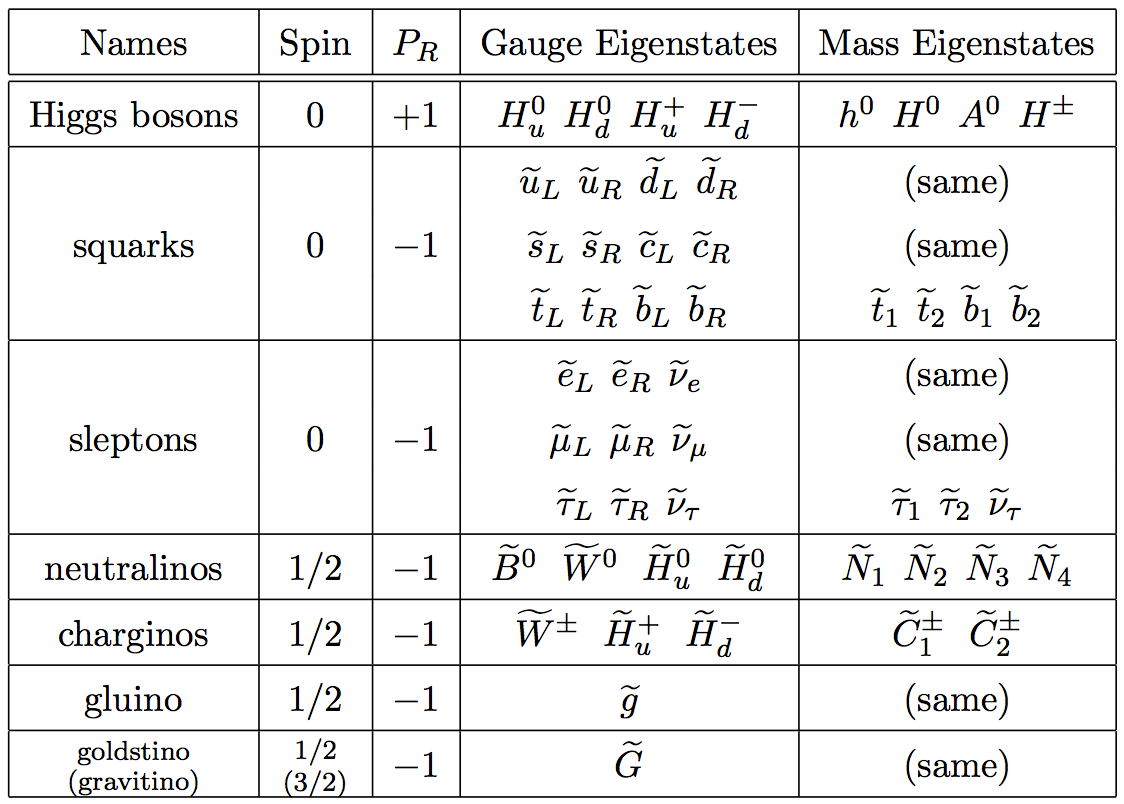
\includegraphics[width=0.75\textwidth]{theory/pics/SUSY_particles_table.png}
		\end{tabular}
		\caption{SUSY particles in MSSM~\protect\cite{Martin:1997ns}}
		\label{fig:SUSY_particles_table}
\end{table}

\FloatBarrier

\subsection{Motivations}

\FloatBarrier

As said before SUSY and all the other models try to explain some of the aspects of Nature that the Standard Model can't include. The following list 

\begin{itemize}
	\item \textbf{Dark Matter candidate}: The assumpition of R-parity conservation prevents the lightest of the SUSY particles, also called LSP, to decay any further into lighter Standard Model particles. In order to fit into the profile of a Dark Matter candidate this particle cannot interact with matter any further, therefore the best choice for the LSP is the lightest neutralino \neutralinoone.  
	
	\item \textbf{Hierarchy problem solution}:  the corrections to the Higgs mass are exactly canceled by the symmetric partners of the Standard Model particles with opposite sign. An example of the top quark correction to the Higgs mass being canceled by a supersymmetric scalar top $\widetilde{t}$ correction is shown in \autoref{fig:higgs_loop}
	
	\begin{figure}[tbh!]
		\centering
		\begin{tabular}{cc}
			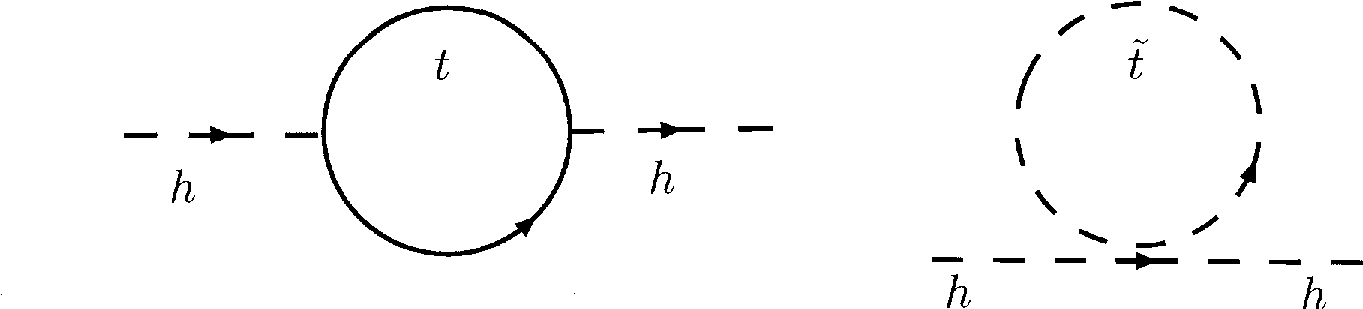
\includegraphics[width=0.75\textwidth]{theory/pics/higgs_loop.png}
		\end{tabular}
		\caption{In SUSY, the correction to Higgs mass by the top quark (L) is inherently cancelled by the contribution from the top quark's supersymmetric partner, the stop (R).}
		\label{fig:higgs_loop}
	\end{figure}

	\item \textbf{Naturalness and parsimony}: Along with the hierarchy problem solution many scientific observation made during the first run of LHC suggest a supersymmetric theory that more naturally explains the weak scale\cite{Craig:2013cxa}. The proposition of a new theory based on the MSSM could also adopt a more "parsimonious" approach. Parsimony involves the inclusion in the theory of additional rules such as assuming there aren't additional fields besides the ones required to promote supersymmetry, considering a high SUSY breaking scale, requiring the colored sparticles to be havier than the uncolored ones, assuming a small number of supersymmetry breaking parameters and finally considering the non-differentiation of the Standard Model generations by the SUSY breaking mechanism. A combination of both naturalness and parsimony leads to a sparticle featuring a low mass ($\approx\gev$) stop $\widetilde{t}$, higgsinos $\widetilde{h}$, electroweakinos $\widetilde{W}$ nad sleptons $\widetilde{l}$ and a high mass ($\approx\tev$) gluino $\widetilde{g}$ and squarks $\widetilde{q}$. A summary of the given SUSY particles mass scales is shown on \autoref{fig:SUSY_naturalness}.

	\begin{figure}[tbh!]
		\centering
		\begin{tabular}{cc}
			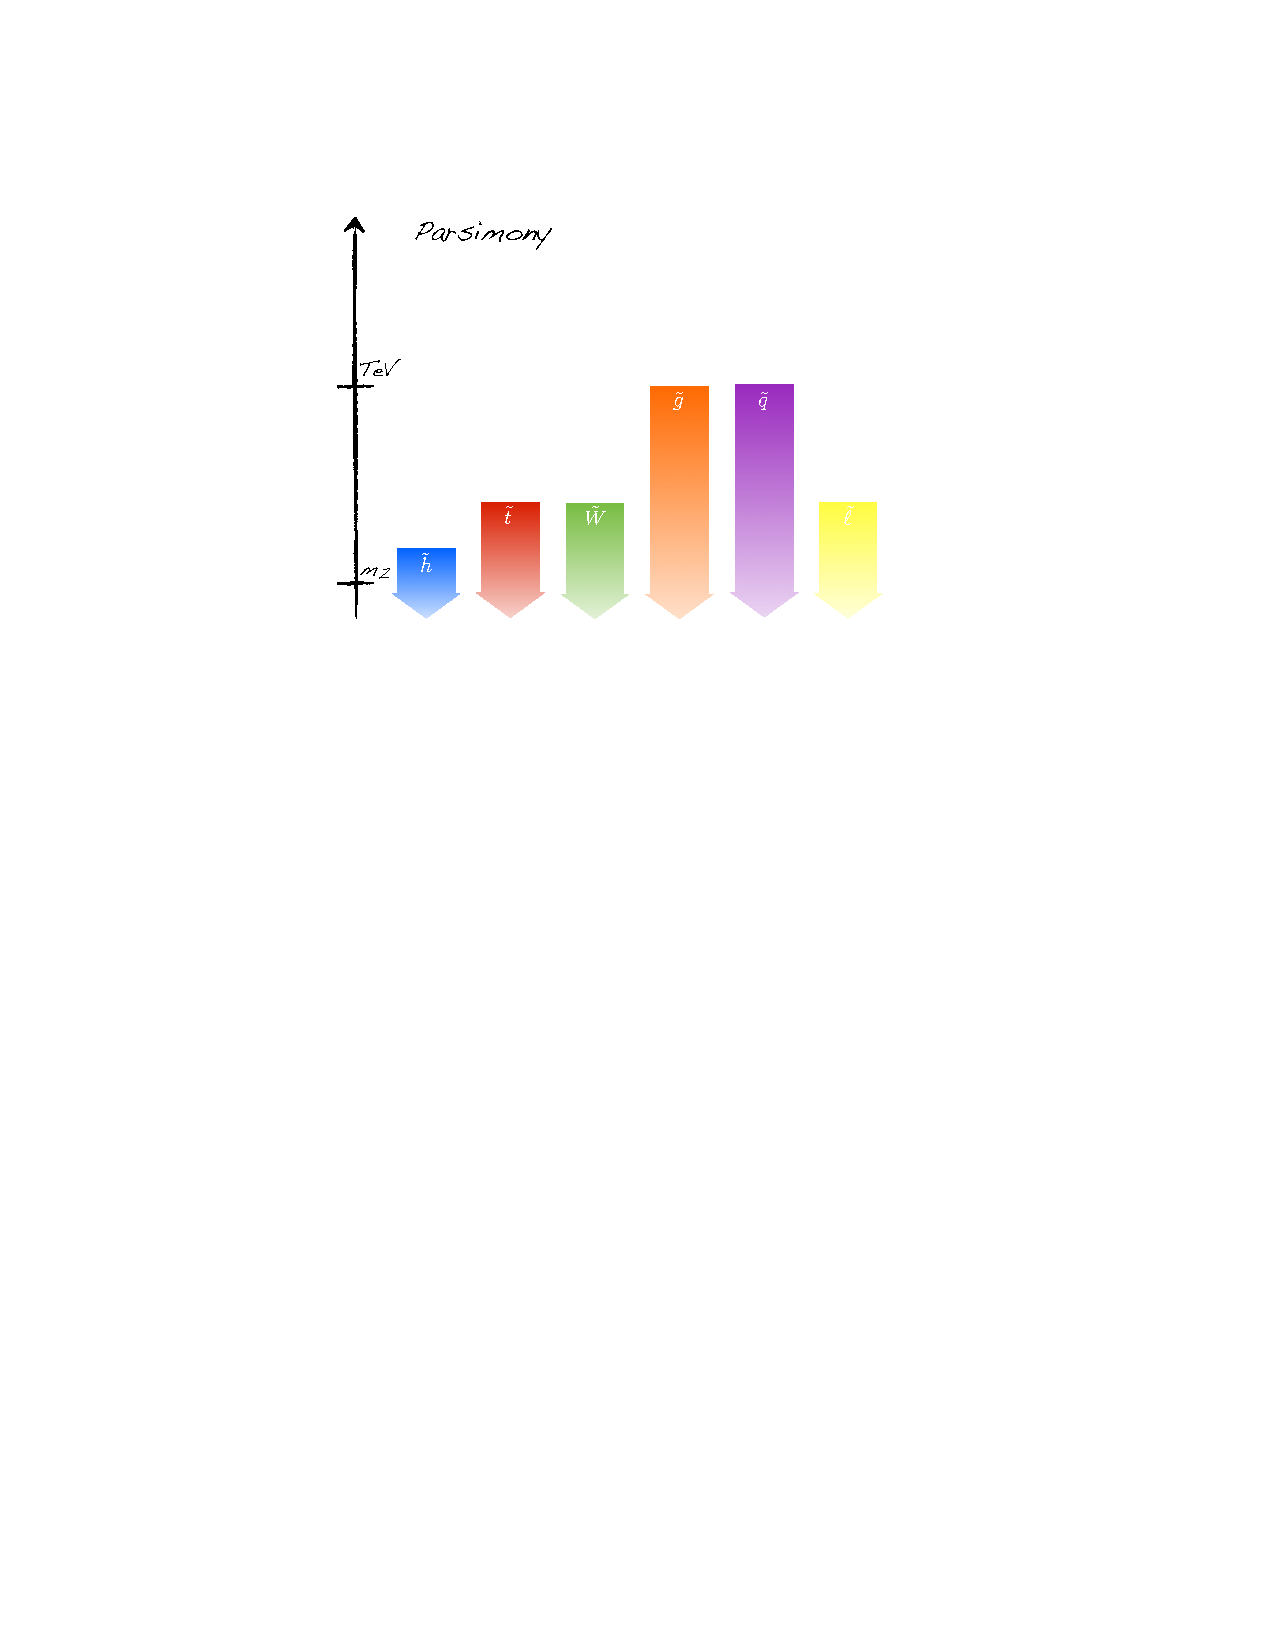
\includegraphics[width=0.75\textwidth]{theory/pics/SUSY_naturalness.pdf}
		\end{tabular}
		\caption{Cartoon illustration of the mass scales for various sparticles dictated solely by electroweak naturalness with sensitivity parameter $\Delta \lesssim 10$.}
		\label{fig:SUSY_naturalness}
	\end{figure}
	
	\item \textbf{Gravity and forces unifications}: supersymmetric models , for example minimal supergravity (mSUGRA)\cite{Ellis:2013oxa},can take take into account a gravity-mediated supersymmetry breaking \cite{Martin:1997ns}, leading to unification of the gauge couplings at the GUT scale. Those assumptions reduces the numbers of MSSM parameters.

\end{itemize}

\FloatBarrier

\subsection{SUSY generic signatures at the LHC with charginos and neutralinos}

\FloatBarrier

The assumptions made by the most important SUSY models set the mass of the first generation charginos \charginopm and next-to-lightest neutralino \neutralinotwo to values not much far from the LSP mass \neutralinoone. The possibility of being the first SUSY particles to be discovered gives the spotlight to this topology of SUSY searches in past literature \cite{Abel:2000vs}. 

In case of a mass split between the LSP and next-to-lightest neutralino \neutralinotwo or the lightest chargino \charginopm largen than $\text{M}_{Z}$ or $\text{M}_{W}$, the particles will decay into massive gauge bosons and the LSP \neutralinoone. If not, the decays will occur through virtual gauge boson and scalar fermion exchanges, leading in the final state to the LSP neutralino and a fermion-antifermion pair. It has been realized \cite{Baer:1998bj, Baer:1998sz, Bartl:1999iw, Djouadi:2000aq} that for large values of the parameter \tanbeta, the ratio of the vacuum expectation values of the two doublet Higgs fields which are needed to break the electroweak symmetry in the MSSM, the Yukawa couplings of third generation down-type fermions (b quarks and $\tau$ leptons), which are strongly enhanced, lead to dramatic consequences for the decays of these particles. Indeed, the virtual exchanges of, on the one side, Higgs particles (because the Higgs boson couplings to b quarks and $\tau$ leptons are proportional to \tanbeta) and, on the other side, of third generation down-type sfermions (which tend to be lighter than the other sfermions in this case) become very important.

Many scenarios has been taken into account for those decays considering different SUSY breaking parameters configuration \cite{Djouadi:2001fa}. 

For example \autoref{fig:br_chitautau} and \autoref{fig:br_chibbarb} show, respectively, the branching ratios $\text{BR}(\neutralinotwo \longrightarrow \neutralinoone\tau^{+}\tau^{-} )$ and $\text{BR}(\neutralinotwo \longrightarrow \neutralinoone b \bar{b})$, as functions of $m_{\widetilde{\tau}1}$ or $m_{\widetilde{b}1}$ for $\mu = 500\gev$ (a), as a function of $\mu$ (b) and as a function of \tanbeta (c) for $m_{0} = 300\gev$. There is an evident competition between $b\bar{b}$ and $\tau^{+}\tau^{-}$ final states. In the case of a light A boson and for large \tanbeta values, the A and h contributions are much more important in the decay $\neutralinotwo \longrightarrow \neutralinoone b \bar{b}$ than in the channel $\neutralinotwo \longrightarrow \neutralinoone\tau^{+}\tau^{-} $ because of the larger b-quark mass and the color factor; the Higgs contribution makes then $\text{BR}(\neutralinotwo \longrightarrow \neutralinoone b \bar{b})$ dominating, except when $\widetilde{\tau}_{1}$ is very light, and the two body decay $\neutralinotwo \longrightarrow \stau \tau$ is close to occur, making $\text{BR}(\neutralinotwo \longrightarrow \neutralinoone\tau^{+}\tau^{-} )$ close to unity. Even for heavy A, and H bosons, $\text{BR}(\neutralinotwo \longrightarrow \neutralinoone b \bar{b})$ can reach the level of 50\%. However, for large enough values of \tanbeta and $\mu$, it is the decay channel $\neutralinotwo \longrightarrow \neutralinoone\tau^{+}\tau^{-} $ which dominates, since for a universal scalar mass $m_{0}$, the stau is always lighter than the $\widetilde{b}_{1}$ state and its virtual contribution is larger, despite of the color factor. The sum of the two branching ratios is in general close to unity.

\begin{figure}[tbh!]
	\centering
	\begin{tabular}{cc}
		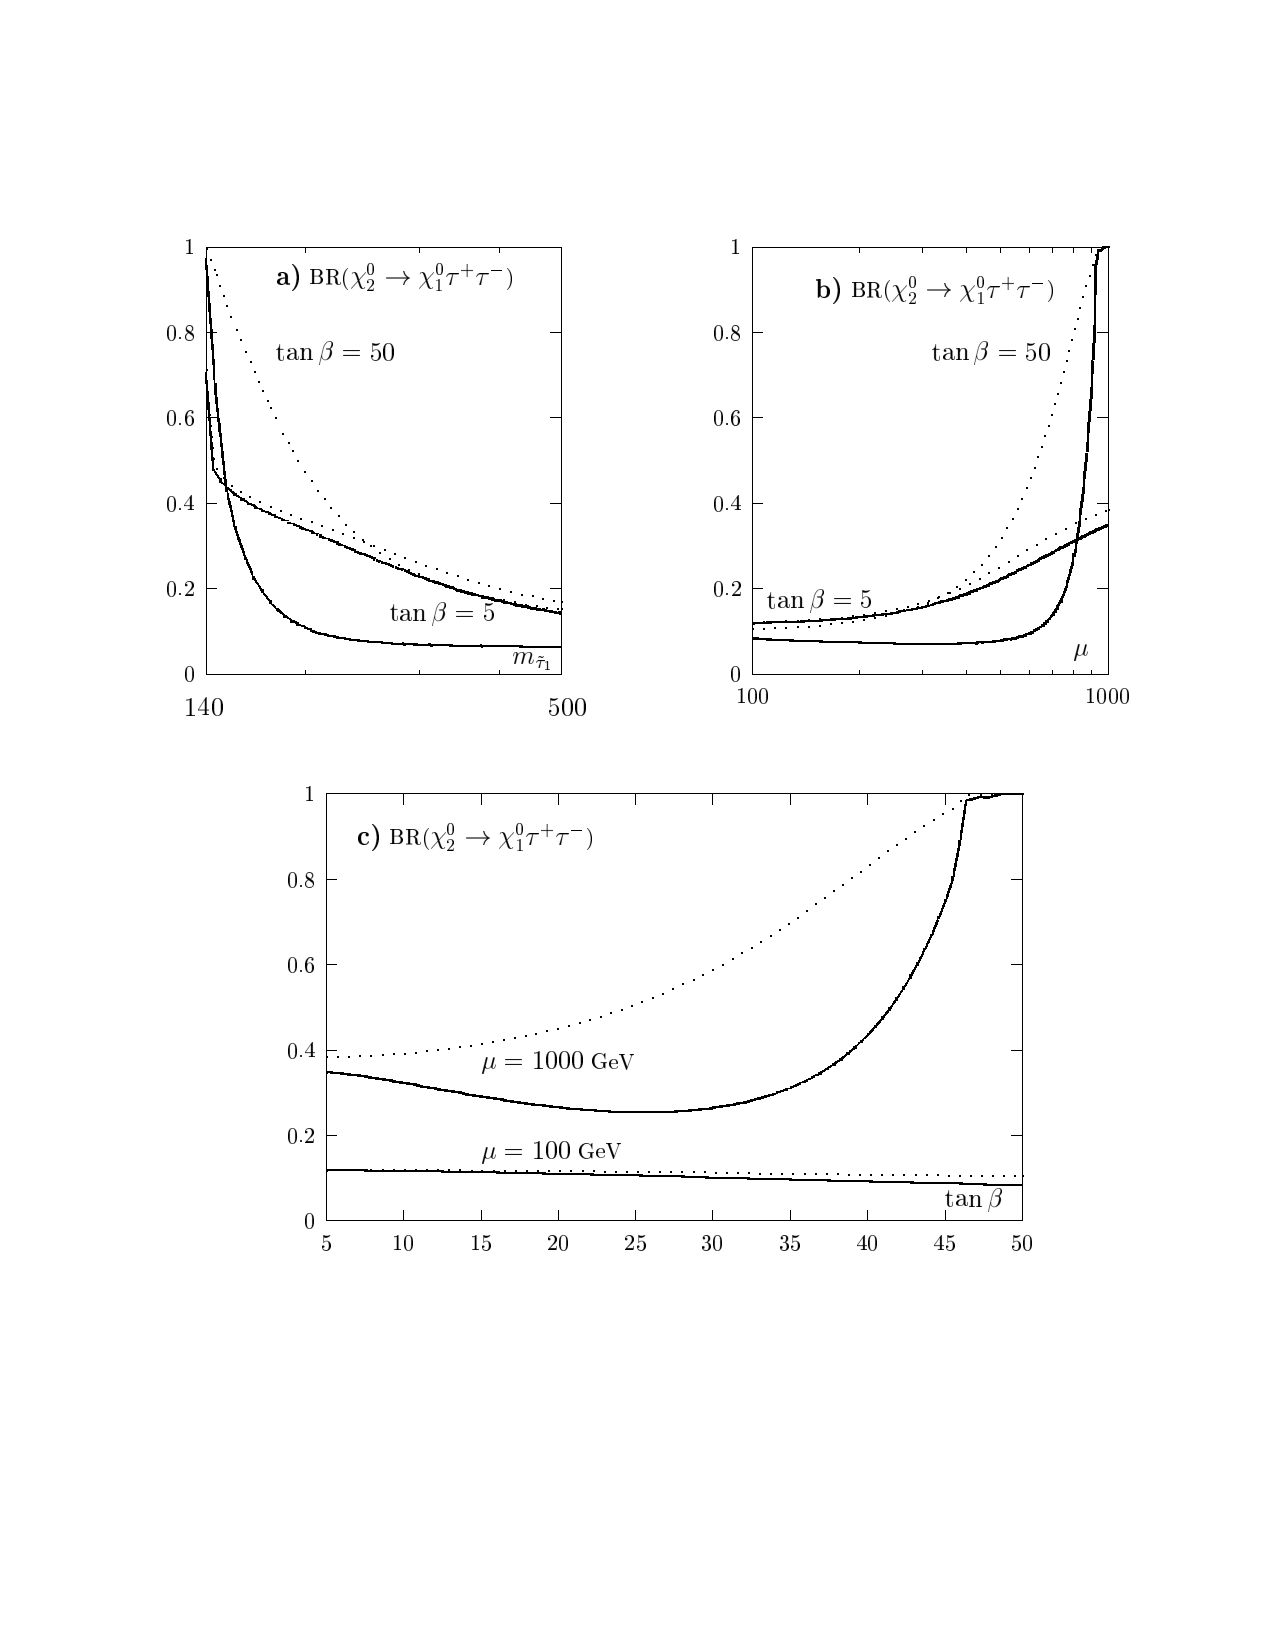
\includegraphics[width=0.80\textwidth]{theory/pics/br_chitautau.pdf}
	\end{tabular}
	\caption{The branching ratio $\text{BR}(\neutralinotwo \longrightarrow \neutralinoone\tau^{+}\tau^{-} )$ for two values of \tanbeta = 5 and 50 and two values of $M_{A} = 100\gev$ (dashed lines) and 500\gev (solid lines) as a function of $m_{\widetilde{\tau}1}$  for $\mu = 500\gev$ (a) as a function of $\mu$ assuming $m_{0} = 300\gev$ (b) and as a functionof \tanbeta for two values of $\mu = 100$ and $1000\gev$ (c); $M_{2}$ is fixed to $150\gev$.}
	\label{fig:br_chitautau}
	
\end{figure}

\begin{figure}[tbh!]
	\centering
	\begin{tabular}{cc}
		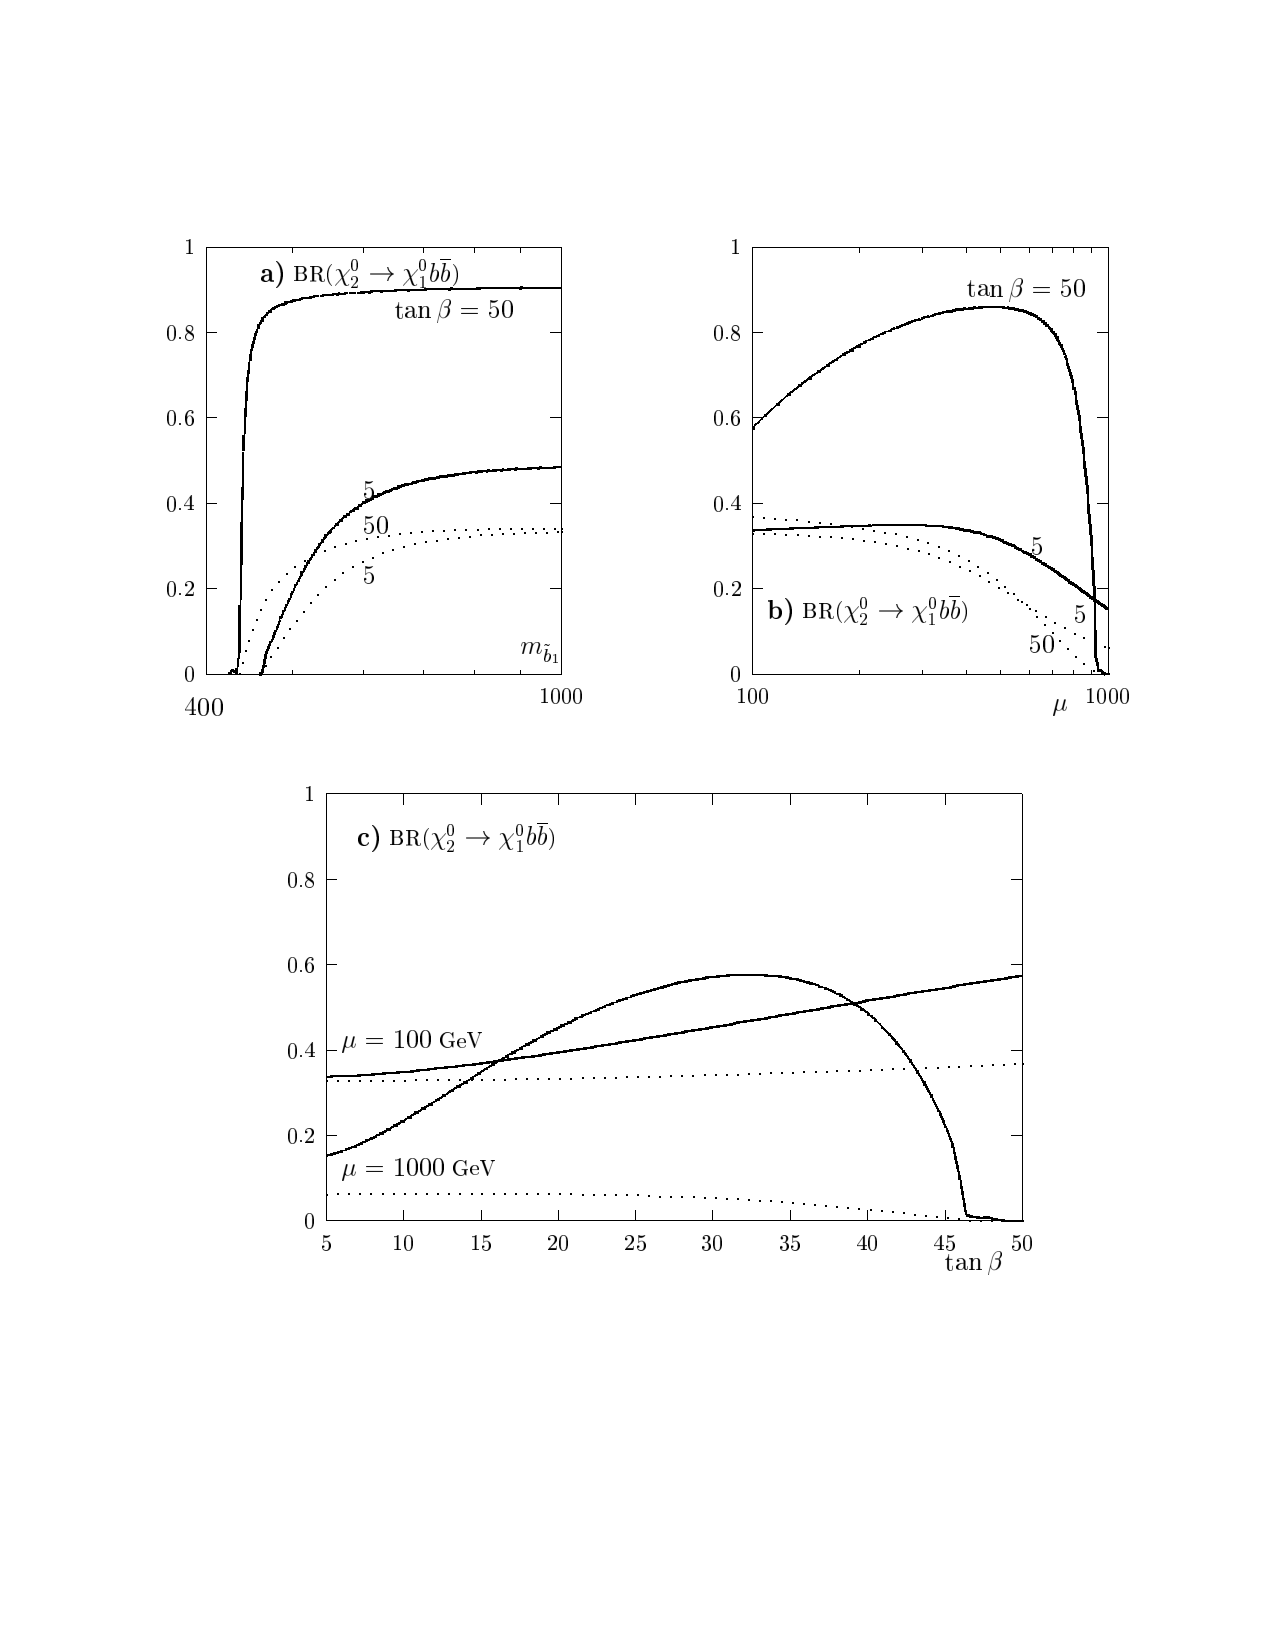
\includegraphics[width=0.90\textwidth]{theory/pics/br_chibbarb.pdf}
	\end{tabular}
	\caption{The branching ratio $\text{BR}(\neutralinotwo \longrightarrow \neutralinoone b \bar{b})$ for two values of $\tanbeta = 5$ and $50$ and two values of $M_{A} = 100\gev$ (solid lines) and $500\gev$ (dashed lines) as a function of $m_{\widetilde{b}1}$ for $\mu = 500\gev $ (a) as a function of $\mu$ assuming $m_{0} = 300\gev$ (b) and as a function of \tanbeta for two values of $\mu = 100$ and $1000\gev$ (c); $M_{2}$ is fixed to $150\gev$.}
	\label{fig:br_chibbarb}
	\end{figure}

\FloatBarrier

\clearpage
